%%%%%%%%%%%%%%%%%%%%%%%%%%%%%%%%%%%%%%%%%%%%%%%%%%%%%%%%%%%%%%%%%%%%%%%%%%%%%%%%%%%%%%%%%%%%%%%%%%%%%%%
%%%%%%%%%%%%%% Template de Artigo Adaptado para Trabalho de Diplomação do ICEI %%%%%%%%%%%%%%%%%%%%%%%%
%% codificação UTF-8 - Abntex - Latex -  							     %%
%% Autor:    Fábio Leandro Rodrigues Cordeiro  (fabioleandro@pucminas.br)                            %% 
%% Co-autor: Prof. João Paulo Domingos Silva  e Harison da Silva                                     %%
%% Revisores normas NBR (Padrão PUC Minas): Helenice Rego Cunha e Prof. Theldo Cruz                  %%
%% Versão: 1.0     13 de março 2014                                                                  %%
%%%%%%%%%%%%%%%%%%%%%%%%%%%%%%%%%%%%%%%%%%%%%%%%%%%%%%%%%%%%%%%%%%%%%%%%%%%%%%%%%%%%%%%%%%%%%%%%%%%%%%%
% \section{\esp Introdução}

% A formatação deverá ter parágrafo recuado a 1,25 centímetros, tamanho 12, fonte Arial ou Times New Roman , espaçamento 1,5 justificado. Todo o texto deverá conter essa formatação com exceção para citações textuais, 
% descritas adiante neste modelo. Os títulos dos capítulos devem utilizar a formatação caixa alta, negrito, tamanho 12.

% \section{\esp Desenvolvimento}

% Todo título de seção ou subseção deverá ser seguido de texto.
% Para as seções textuais utilizar numeração progressiva em algarismos arábicos, limitada até a seção quinária 
% (NBR 6024/2003) da ABNT. Devem ser diferenciadas utilizando os recursos gráficos abaixo \cite{manualpuc}.
% Os títulos das seções primárias devem ser em caixa alta, negrito, tamanho 12.

\section{\esp Introdução \label{introducao}}

%considerações iniciais
O \ac{SAD} caracteriza-se como uma modalidade de assistência à saúde prestada em domicílio composta por um conjunto de ações de prevenção, reabilitação e tratamento de doenças.
Esse tipo de serviço tem se tornado cada vez mais presente, oferecendo uma forma alternativa de atendimento às pessoas com quadro clínico estável e que necessitam de cuidados especializados, substituindo a internação hospitalar.

Essa modalidade de assistência a saúde oferece maior comodidade aos pacientes, garantindo maior conforto, facilitando o apoio familiar, além de reduzir riscos de contaminação hospitalar e a lotação dos leitos nos hospitais.
Por outro lado, o~\ac{SAD} apresenta alguns desafios para os profissionais de saúde, tais como a necessidade de deslocamento dos profissionais de saúde de forma  que todos os pacientes que estejam agendados para determinado dia sejam atendidos no tempo previsto, além do complexo planejamento das escalas de trabalho dos profissionais de saúde envolvidos no atendimento domiciliar \cite{Kergosien:2009}. 
Visando atender pacientes em domicílio, é necessário definir rotas a serem seguidas pelos veículos do~\ac{SAD}, pois os caminhos a serem percorridos podem depender de alguns fatores, tal como a necessidade de urgência de algum paciente. 

Devido ao complexo planejamento das escalas de trabalho dos profissionais e as dificuldades encontradas para completar todo o serviço diário no tempo previsto, sem exceder a carga horária dos profissionais de saúde, o \ac{SAD} tem despertado o interesse de diversos pesquisadores. Dessa forma, o problema relacionado à modalidade estudada foi definido como \ac{PERE}.
O \ac{PERE} aborda de forma integrada o problema de roteamento de veículos e de escalonamento de enfermeiras, com o objetivo de desenvolver um cronograma de trabalho para o \ac{SAD}, de forma que cada enfermeira visite um conjunto de pacientes, faça uma pausa e finalize suas atividades previstas dentro de uma janela de tempo de trabalho pré definida \cite{trabelsi:2012}. 
Para satisfazer as restrições do \ac{PERE}, além de definir a escala de trabalho dos profissionais, é necessário definir rotas que serão seguidas pelos veículos do \ac{SAD}, uma vez que a elaboração dos trajetos dependem de alguns fatores, tal como a necessidade de urgência de algum paciente. 

%Segundo \cite{Kergosien:2009} é possível reduzir o PERE ao Problema dos Múltiplos Caixeiros Viajantes, dessa forma, pode-se classificar o \ac{PERE} na classe de problemas NP-Difícil, portanto, é pouco provável que seja possível determinar um algoritmo polinomial para resolve-lo.
Segundo \citeonline{Kergosien:2009} é possível reduzir o PERE ao Problema dos Múltiplos Caixeiros Viajantes, classificando-o na classe de problemas NP-Difícil. Portanto, é pouco provável que seja possível determinar um algoritmo polinomial para resolve-lo.
Apesar disso, de acordo com \citeonline{cheng:98}, \citeonline{bachouch:2010},\citeonline{tozlu:2016} e \citeonline{cattafi:2012}, o \ac{PERE} ainda é resolvido de forma manual em diversos países, o que pode acarretar em resultados insatisfatórios. 
Por fim, é estimado em \citeonline{holm:2014} que os profissionais envolvidos no \ac{SAD} passam entre $18\%$ e $26\%$ da sua jornada de trabalho dentro do veículo realizando translados entre os pontos de atendimento, o que reforça a necessidade da utilização de técnicas de otimização.

Devido a natureza do problema, diversos métodos para determinar a melhor solução para o \ac{PERE} são encontrados na literatura. Com o objetivo de investigar de maneira formalizada, quais métodos vêm sendo desenvolvidos para solucioná-lo, encontrar  possíveis problemas de investigação existentes, garantindo a replicabilidade desta revisão e  auxiliando outros pesquisadores do tema no momento da obtenção de materiais de estudo, elaboramos uma \ac{RSL}.
%Para verificar a necessidade da elaboração de uma \ac{RSL}, foram elaboradas pesquisas para buscar a existência de outra revisão da mesma natureza. 
Nas pesquisas realizadas não foram encontradas outras \ac{RSL}, mas foram encontradas outras revisões de literatura, classificadas por \citeonline{Kitchenham:2007} como revisão ad-hoc,  publicadas por \citeonline{fikar:2017} e \citeonline{mohamed:2017}.

%organização do artigo

Este artigo está organizado da seguinte forma:  Na Seção~\ref{protocolo} é apresentado o protocolo da revisão sistemática de literatura. Na Seção~\ref{terminologia}  são apresentadas as terminologias relacionadas ao PERE que são utilizadas também ao longo do texto. Na Seção~\ref{pad} são apresentadas as métricas utilizadas para avaliar as soluções do \ac{PERE}. Na Seção~\ref{metodologia}  foram descritas as metodologias mais utilizadas. Na Seção~\ref{aplicacoes} são apresentados os comparativos do \ac{PERE} com outros problemas. Na Seção~\ref{casos} listamos alguns estudos de casos e discutimos alguns problemas com características únicas, e finalizando o artigo, na Seção~\ref{conclusão} são apresentadas as considerações finais.

\section{\esp Protocolo da Revisão Sistemática de Literatura }\label{protocolo}

%Definição, diferença
Segundo \citeonline{Kitchenham:2007}, uma \ac{RSL} é um método de seleção de artigos, no qual a busca por materiais bibliográficos é formalizada sistematicamente a partir da elaboração e utilização de um protocolo de busca. Uma \ac{RSL} tem como objetivos: resumir evidências empíricas, identificar lacunas existentes nas pesquisas realizadas até o momento e fornecer subsídios para realizar novas pesquisas.
Enquanto uma Revisão Literatura, também chamada de Revisão Ad-hoc, não utiliza o protocolo para a formalização da pesquisa realizada, dessa forma tornando mais difícil sua replicabilidade.

%etapas
\citeonline{Kitchenham:2007} afirmam que uma \ac{RSL} é  composta por três fases: planejamento da revisão, condução da revisão e análise dos materiais obtidos.
Na fase de planejamento define-se a pergunta de pesquisa, seleciona-se as palavras chave e determina-se os critérios de inclusão e de exclusão de materiais bibliográficos; na condução da revisão é realizado uma busca a partir da combinação das palavras chave e na última fase  é realizado um estudo dos materiais que foram obtidos. A seguir será apresentada a descrição das etapas da elaboração e a execução do protocolo de \ac{RSL} utilizado neste artigo para encontrar e selecionar os materiais que posteriormente foram estudados neste artigo.

%Protocolo da revisão
\subsection{Planejamento da Revisão}

A \acl{RSL} proposta neste trabalho tem como objetivo investigar quais métricas e metodologias aplicadas ao \ac{PERE} entre 1998 e o mês de Outubro de 2016, de forma a responder a seguinte questão de pesquisa:

\begin{itemize}
\item \emph{Quais métricas e metodologias empregadas ao \acl{PERE} foram publicadas desde 1998 até o mês de Outubro de 2016?}
\end{itemize}

Para responder à pergunta foram consultados artigos de pesquisadores que aplicaram métricas e metodologias ao \ac{PERE}, tendo como um dos resultados esperados a relação das métricas e metodologias utilizadas no período de tempo definido na questão anterior. 

A consulta por artigos relacionados foi realizada com a utilização das seguintes palavras chave:

\begin{itemize}
\item \textit{``home health care''}
\item \textit{``home care''}
\item \textit{``nurse''}
\item \textit{``routing''}
\item \textit{``scheduling''}
\end{itemize}

Organizadas na seguinte expressão de busca:

\begin{itemize}
\item \textit{`` ( (``home health care'' OR ``home care'' OR ``nurse'') AND ``routing'' AND ``scheduling'' ) ''}
\end{itemize}

Após a elaboração da expressão de busca, foram definidos os critérios para inclusão e exclusão dos materiais bibliográficos, de acordo com a Tabela \ref{inclusao}.

% \textbf{Critérios de inclusão:}
% \begin{itemize}
% \item Artigos relacionados ao Problema de Escalonamento e Roteamento de Enfermeiras; 
% \item Artigos publicados em revistas ou conferências;
% \item Artigos completos.
% \end{itemize}

% \textbf{Critérios de exclusão:}

% \begin{itemize}
% \item Artigos que foram publicados em idiomas que diferem do inglês ou português;
% \item Artigos inacessíveis ou indisponíveis;
% \item Artigos duplicados;
% \item Artigos publicados antes de 1998.
% \end{itemize}

\begin{table}[H]
\centering
\caption{Critérios para inclusão ou exclusão de artigos}
\label{inclusao}
\begin{tabular}{@{}L{6cm}|L{8cm}@{}}
 \hline
 \multicolumn{1}{c|}{\textbf{Critérios de inclusão}}                                                                       & \multicolumn{1}{c}{\textbf{Critérios de exclusão}}                                                                      \\ \hline
 \begin{tabular}[c]{@{}l@{}}- Artigos relacionados ao \ac{PERE}\end{tabular} & \begin{tabular}[c]{@{}l@{}}- Artigos que foram publicados em idiomas\\  que diferem do inglês ou português\end{tabular} \\ \hline
 - Artigos publicados em revistas ou conferências                                                                          & - Artigos inacessíveis ou indisponíveis                                                                                 \\ \hline
 - Artigos completos                                                                                                       & - Artigos duplicados                                                                                                    \\ \hline
 \multicolumn{1}{c|}{-----}                                                                                                & - Artigos publicados antes de 1998                                                                                      \\ \hline
 \end{tabular}
\\ \textbf{\footnotesize Fonte: Autoria Própria } 
\end{table}

\subsection{\esp Condução das buscas}

Após a definição dos critérios de inclusão e de exclusão dos materiais bibliográficos, foram escolhidas as seguintes bases de pesquisa, a partir da sua popularidade, para realizar as buscas:

\begin{itemize}
\item \textit{Science Direct};
\item \textit{Springer};
\item \textit{Scopus};
\item \textit{IEEE Xplore};
\item \textit{ACM Digital Library}.
\end{itemize}

Após a realização das buscas, foram retornados 158 resultados, organizados na Figura~\ref{bases}. 

\begin{figure}[ht]
\begin{center}
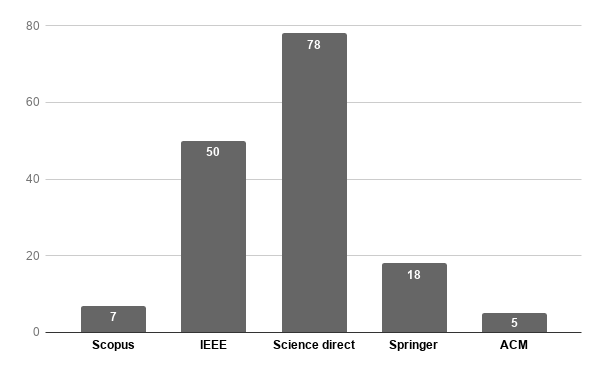
\includegraphics[width=0.6\textwidth]{base_de_dados_de_origem.png}
\caption{Contagem por bases de pesquisa \label{bases} \\ \textbf{\footnotesize Fonte: Autoria Própria (2018)}}
\end{center}
\end{figure}


A partir da aplicação dos critérios de inclusão e de exclusão nos artigos consultados foram aceitos 19 artigos, por atenderem a todos os critérios de inclusão e 139 artigos rejeitados por atenderem a pelo menos um critério de exclusão ou por não se encaixarem em algum critério de inclusão. É interessante observar que os artigos coletados foram publicados entre os anos de 1998 e 2016, sendo que houve um aumento considerável de publicações entre os anos de 2012 e 2016, de acordo com a Figura~\ref{ano}.
 
Após a aplicação dos critérios de inclusão e exclusão nos materiais bibliográficos, foi observado que 86,7\%  dos artigos foram rejeitados. Acredita-se que o motivo para este alto índice de rejeição seja por conta da relação do assunto estudado com publicações existentes em diversas áreas de saúde, fazendo com que as bases de pesquisa apontassem para artigos que posteriormente não se encaixariam em algum critério de inclusão. 

\begin{figure}[!h]
\begin{center}
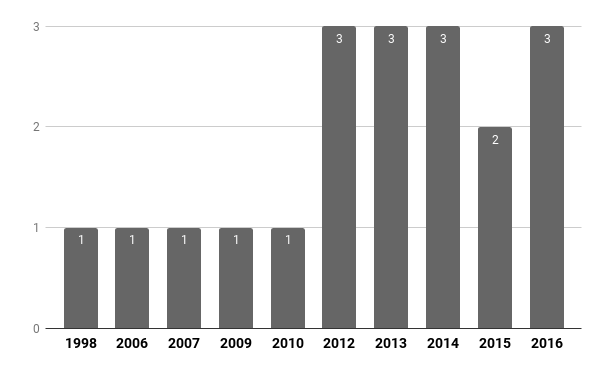
\includegraphics[width=0.6\textwidth]{contagem_por_ano.png}
\caption{Contagem de artigos por ano de publicação 
\\ \textbf{\footnotesize Fonte: Autoria Própria (2018)}}
\label{ano}
\end{center}
\end{figure}

%ok
Duas revisões ad-hoc, encontradas na fase de análise de materiais obtidos, desenvolvidas por \citeonline{mohamed:2017} e \citeonline{fikar:2017}, merecem destaque. Segundo \citeonline{Kitchenham:2007}, esses trabalhos são classificados como revisões de literatura ad-hoc, pois não foram elaborados seguindo um protocolo formal para realizar a busca dos materiais, possuem objetivos abrangentes, não possuem uma questão de pesquisa a ser respondida ao final da revisão, não foram elaboradas expressões de busca nem critérios para inclusão e exclusão para filtrar os estudos retornados na pesquisa. 

A partir dos resultados obtidos em sua revisão, foi afirmado por \citeonline{fikar:2017} que o \ac{PERE} foi primeiro estudado em 1974 a partir do artigo \textit{A Model for Community Nursing in a Rural County}, publicado por \citeonline{fernandez:1974}. Em suas pesquisas \citeonline{fikar:2017}, verificaram  que alguns artigos estão diretamente relacionados com o \ac{PRV} e que as restrições mais consideradas incluem janelas de tempo, requisitos de habilidades e de tempo de trabalho. 

%\citeonline{fikar:2017} compararam diferentes objetivos, restrições e destacar as pesquisas futuras para o \ac{PERE}, para isto os autores revisaram diversos artigos, até Outubro de 2015, não indicando a data do início da sua pesquisa. %As buscas foram realizadas pelos autores a partir seguintes palavras chave: \textit{``Home Care'', ``Home Health Care'', ``Routing'' e ``Scheduling''}. 



%A revisão de literatura desenvolvida por \citeonline{mohamed:2017} tem como objetivo analisar a literatura existente relativa ao \ac{PERE}, %para isso o autor comparou  materiais de diferentes naturezas, tais como artigos científicos, capítulos de livros, teses, dissertações e relatórios técnicos, publicados entre 1997 e 2015, a partir das seguintes palavras chave: \textit{ ``Home Health Care'', ``Home Care'' ``Resource  Scheduling'',  ``Routing'' e ``Vehicle Routing Problem"}


%\citeonline{fikar:2017} destacaram, as seguintes técnicas de solução aplicadas ao \ac{PERE}: \textit{Adaptative Large Neighborhood Search, Variable Neighborhood Search, Branch and Price and cut, Discrete-Event-Simulation, Greedy Randomized Adaptive Search Procedure, Fuzzy Simulated Evolution Algorithm, Genetic Algorithm, Memetic Algorithm, Multi-Directional Local Search, Particle Swarm Optimization, Repeated Matching, Simulated Annealing, Scatter Search e Tabu Search}.

%Adicionar a tabela

%\citeonline{mohamed:2017}, em sua revisão de literatura, não se limitou somente à análise de artigos e incluiu outras fontes de conhecimento \footnote{melhorar!}.
Além de artigos científicos, \citeonline{mohamed:2017} incluiu em sua revisão de literatura materiais obtidos  de outras fontes, tais como: livros, relatórios técnicos e dissertações.
Outra contribuição de \citeonline{mohamed:2017} foi a classificação das restrições relacionadas aos pacientes, a organização e aos profissionais como: temporais, de associação e geográficas, de acordo com a Tabela \ref{classificacao1}. 


\begin{table}[h]
\centering
\caption{Classificação do esquema baseado em restrições}
\label{classificacao1}
\begin{tabular}{@{}C{2cm}|L{5cm}L{4cm}L{4.5cm}@{}}
\hline
\multirow{2}{*}{\textbf{Atores}}  & \multicolumn{3}{c}{\textbf{Restrições}}                                                                                                                 \\ \cline{2-4} 
                                       & \multicolumn{1}{c|}{\textbf{Temporal}} & \multicolumn{1}{c|}{\textbf{Atribuição}} & \multicolumn{1}{c}{\textbf{Geográfica}}                             \\ \hline
\multirow{2}{*}{\textbf{Empresa}}      & - Período de planejamento              & - Continuidade do serviço            & - Setores/distritos                                                 \\
                                       & - Frequência da decisão de roteamento  &                          & - Tipologia dos serviços prestados pelo \ac{PERE} \\ \hline
\multirow{4}{*}{\textbf{Pacientes}}    & - Frequência das visitas               & - Preferências                         & - Localização do paciente                                        \\
                                       & - Janela de tempo                      &                                          &                                                                     \\
                                       & - Dependências temporais               &                                          &                                                                     \\
                                       & - Serviços disjuntos                   &                                          &                                                                     \\ \hline
\multirow{2}{*}{\textbf{Profissional}} & - Tipo de contrato                     & - Qualificação                           & - Localização das enfermeiras                                       \\
                                       & - Horas trabalhadas                    & - Balanceamento de carga horária         &                                                                     \\ \hline
\end{tabular}
\\ \textbf{\footnotesize Fonte: \citeonline{mohamed:2017} } 
\end{table}

Para as empresas, as restrições temporais referem-se ao período de planejamento da empresa e por quanto tempo este planejamento é válido; as restrições de atribuição são utilizadas para garantir a continuidade dos atendimentos até o final do tratamento; as restrições geográficas são utilizadas para determinar a área de abrangência do serviço.
Para os pacientes, as restrições temporais são utilizadas para determinar quantas visitas serão realizadas durante determinado período de tempo, a janela de tempo, determina o limite superior e inferior para o início do atendimento e as dependências temporais determinam a duração das visitas e por quanto tempo o serviço será oferecido; as restrições de associação determinam as preferências dos pacientes, tais como: ser atendido sempre pela mesma enfermeira; as restrições geográficas estão associadas a localização do paciente, sendo utilizado para determinar se este está dentro da área de atuação da empresa, além de auxiliar no cálculo de estimativa de tempo de viagem.
Para os profissionais, as restrições temporais são utilizadas determinar sua carga horária de atendimento; as restrições de associação são utilizadas para classificar as habilidades de cada enfermeira e reduzir a quantidade de horas extras trabalhadas; e as restrições temporais são utilizadas para determinar o local de cada atendimento.

Além da Revisão Sistemática de Literatura, este artigo traz como contribuição materiais não retornados por \citeonline{mohamed:2017} e \citeonline{fikar:2017}, além de enfatizar estudos de caso investigados em conjunto com empresas e destacar as métricas e metodologias mais empregadas por pesquisadores para solucionar o \ac{PERE}.

\section{\esp Definições e Terminologias}\label{terminologia}

Nesta seção será apresentada a definição e as terminologias do \ac{PERE}. Utilizaremos o termo enfermeira para designar todos os profissionais de saúde envolvidos no \ac{PERE}. 

O Problema de Escalonamento e Roteamento de Enfermeiras é definido por \citeonline{rasmussenm:2012} da seguinte forma: seja $E = \{ e_1, e_2, \ldots, e_{|E|} \}$ um conjunto de enfermeiras no qual cada enfermeira $e\in E$ possui uma carga horária de trabalho $CH_e$, $P = \{p_1, p_2, \ldots, p_{|P|} \}$ um conjunto de pacientes, $S$ um conjunto de serviços $S = \{ s_1, s_2, \ldots, s_{|S|} \}$ e $D_{|P|\times |P|}$ uma matriz de distância. 

Seja $\Delta$ um conjunto de pares ordenados de instantes de tempo nos quais cada elemento $[i_p, f_p] \in \Delta$ caracteriza uma janela de tempo. O instante de tempo $i_{p}$ representa o limite inferior de tempo para iniciar o atendimento ao paciente $p$ e $f_{p}$ representa o limite superior de tempo iniciar o atendimento ao paciente $p$. A função $f: S \rightarrow \Delta$ mapeia cada serviço de saúde a uma janela de tempo de atendimento. Cada visita realizada a um paciente $p$ deve acontecer dentro de uma janela de tempo $[i_{p},f_{p}]$, sendo que o serviço prestado pela enfermeira $e$ ao paciente $p$ tem a duração máxima definida por $t_s$, associado ao serviço $s \in S$.

Segundo \citeonline{tricoire:2016}, dado o conjunto $E$ de enfermeiras e o conjunto $S$ de serviços solicitados por um ou mais pacientes. 
O \ac{PERE} tem como objetivo encontrar uma rota para cada veículo e um escalonamento para cada enfermeira do \ac{SAD}, indicando quais tarefas devem ser cumpridas por cada enfermeira, em qual ordem e em qual momento, de forma a não ultrapassar a carga horária máxima prevista em lei.
Cada paciente $p\in P$ pode requisitar um ou mais serviços $s \in S$ que serão executados pela enfermeira $e \in E$  com a qualificação necessária para executar determinado serviço $s \in S$. 
% Além de considerar os locais e os pacientes a partir da mesma variável, \citeonline{Bierwirth:2013} considerou em seu trabalho as enfermeiras e os veículos a partir da utilização da mesma variável, uma vez que existe um veículo para cada enfermeira, ou para cada conjunto de enfermeiras que possuem a mesma qualificação.

As rotas do \ac{PERE} podem ser modeladas a partir de um grafo  $G = (V, A)$ no qual $V= \{ v_0, v_1, \ldots, v_{|V|} \}$ é um conjunto de vértices, tal que o vértice $v_0$ representa o local de partida e de chegada das enfermeiras e os demais representam os locais de atendimento. O conjunto de arestas $A = \{(i,j): i\in V, j \in V, i \neq j\}$ representa o translado entre dois locais. 
Cada aresta possui um custo associado $c_{ij}$, representando o tempo de translado entre $v_i$ e $v_j$.
Na Figura \ref{grafo1}, é apresentado o exemplo de uma instância, contendo duas rotas, representando o caminho percorrido por cada enfermeira, que parte de $v_0$, realiza uma série de visitas e retorna ao vértice $v_0$.

\begin{figure}[H]
\centering
\begin{center}
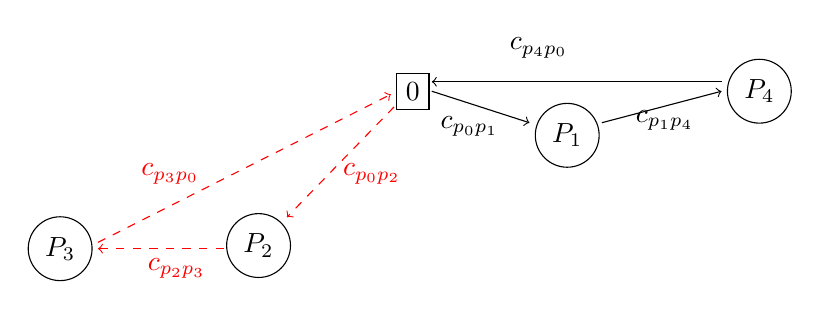
\begin{tikzpicture}[scale=0.4]
	%ponto central
	\draw node[draw] at (0, 0) {$0$};

	%rora 1
   \draw[->, black] (1.8, -0.5) node[below] {$c_{p_0p_1}$} (0.6, 0) -- (3.7, -1.0);
   \draw node[draw, circle] at (4.9, -1.4) {$P_1$};

   \draw[->, black]  (8, -0.3) node[below] {$c_{p_1p_4}$}  (6, -1) -- (9.8, 0);
   \draw node[draw, circle] at (11, 0) {$P_4$};
   
   \draw[->, black] (4, 2) node[below] {$c_{p_4p_0}$} (9.8, 0.3) -- (0.6, 0.3);

	%rota 2
   \draw[->, dashed, red] (-1.3, -2) node[below] {$c_{p_0p_2}$} (-0.6, -0.5) -- (-4, -4);
   \draw node[draw, circle] at (-4.9, -4.9) {$P_2$};
   
   \draw[->, dashed, red] (-7.5, -5) node[below] {$c_{p_2p_3}$} (-6, -5) -- (-10, -5);
   \draw node[draw, circle] at (-11.2, -5) {$P_3$};
   
   \draw[->, dashed, red] (-7.7, -2) node[below] {$c_{p_3p_0}$} (-10, -4.8) -- (-0.7, -0.1);
   
   );
\end{tikzpicture}
\end{center}
\caption{Exemplo de rotas elaboradas para dois veículos do \ac{SAD} 
\\ \textbf{\footnotesize Fonte: Autoria Própria (2018)}
}
\label{grafo1}
\end{figure}


A parte da solução do \ac{PERE} referente ao escalonamento das enfermeiras, pode ser representada a partir de uma matriz $M_{|P|\times |S|}$, na qual cada célula $m_{p_i,s_j} \in M$ contém a atribuição de cada paciente a um ou mais serviços previamente requisitados, como pode ser visto na Tabela \ref{paciente_serviço}.
E uma matriz $M_{|E|\times |S|}$, na qual cada célula $m_{e_i,s_j} \in M$ contém a atribuição de cada enfermeira ao serviço no qual está apta a executar, como pode ser visto na Tabela \ref{enfermeira_serviço} um exemplo com quatro pacientes que requisitam dois serviços e são atendidos pelas enfermeiras qualificadas.

Cada atribuição é definida a partir dos valores $0$ e $1$, sendo o valor $1$ representa que o paciente requisitou o serviço ou que a enfermeira está apta para realizar determinado serviço e $0$ caso contrário. \\


\begin{table}[h]
\centering
\caption{Exemplo da atribuição de pacientes a serviços \label{paciente_serviço}}
\begin{tabular}{c|c|l}
   & s1 & s2	\\ \hline
p1 & 1  & 0     \\ \hline
p2 & 0  & 1      \\ \hline
p3 & 0  & 1     \\ \hline
p4 & 1  & 0     \\ \hline
\end{tabular}
{\footnotesize\\ \textbf{Fonte: Autoria Própria (2018)}}
\end{table}


\begin{table}[H]
\centering
\caption{Exemplo da atribuição de enfermeiras a serviços \label{enfermeira_serviço}}
\begin{tabular}{c|c|l}
   & s1 & s2 \\ \hline
e1 & 0  & 1   \\ \hline
e2 & 1  & 0   \\ \hline

\end{tabular}
{\footnotesize\\ \textbf{Fonte: Autoria Própria (2018)}}
\end{table}




\section{\esp Métricas }\label{pad}

A seguir são descritas algumas métricas utilizadas como medida de qualidade de soluções para o \ac{PERE}.

\subsection{Equilíbrio de Carga Horária}

Um dos desafios do \ac{PERE} é organizar as visitas que devem ser realizadas por cada enfermeira, de forma que a quantidade de horas trabalhadas não exceda a carga horária máxima estabelecida pela legislação trabalhista e a carga de trabalho seja igualmente distribuída.

Sejam $P_{max}$ e $P_{min}$ os limites superiores e inferiores, respectivamente, das cargas horárias de trabalho de uma enfermeira. O balanceamento de carga horária de trabalho é definido em \citeonline{bachouch:2010} pela seguinte função objetivo: 

\begin{center}
$Min~P_{max} - P_{min}$
\end{center}


Foram apresentados por \citeonline{trabelsi:2012} e \citeonline{bachouch:2010}  modelos de \ac{PLI} tendo como objetivo minimizar discrepância da carga horária de trabalho das enfermeiras, sendo considerados cenários com no máximo três enfermeiras por \citeonline{trabelsi:2012} e com no máximo cinco enfermeiras envolvidas por \citeonline{bachouch:2010}. 
\citeonline{Decerle:2016}  atribuíram um custo a cada hora de trabalho e buscaram minimizar o somatório das horas trabalhadas por cada uma das as enfermeiras, também utilizando um modelo de \ac{PLI}. 
Já \citeonline{cheng:98} elaboraram um modelo de \ac{PLI} com o objetivo de minimizar a quantidade de horas extras de trabalho das enfermeiras. Os mesmos autores propuseram uma heurística gulosa construtiva e obtiveram soluções ótimas para diversas instâncias do problema, sendo consideradas no máximo quatro enfermeiras. 

Foi utilizado o método \textit{Branch‐and-Price‐and‐Cut} para resolver problemas de \acl{PLI} por \citeonline{trautsamwieser:2014}. O modelo proposto pelos autores tem como objetivo minimizar o tempo total trabalhado das enfermeiras. Com esta abordagem foram obtidas soluções ótimas para instâncias em cenários com no máximo duas enfermeiras.  

Foi utilizado por \citeonline{mutingi:2013} uma meta-heurística enxame de partículas para reduzir a diferença entre a carga horária de cada enfermeira pelo valor médio da carga horária de todas as enfermeiras. A técnica proposta foi avaliada utilizando instâncias com até 15 enfermeiras, porém não foi apresentada uma discussão profunda dos resultados obtidos. 

Por fim, \citeonline{luna:2013} buscaram minimizar simultaneamente o número de enfermeiras envolvidas no planejamento e a carga horária total diária. Para isso foi utilizado um algoritmo evolucionário paralelizado, sendo capaz de resolver instâncias com até 32 enfermeiras e mais de 10000 serviços prestados, no entanto os autores não apresentam um estudo da optimalidade das soluções obtidas.

\subsection{Maximização de Satisfação}

Uma forma de tornar o atendimento do \ac{SAD} mais agradável é buscar atender, quando possível, as preferências dos pacientes e das enfermeiras. No contexto do \ac{PERE} estas preferências são tratadas como restrições flexíveis, ou seja, que podem ser violadas caso necessário, porém é desejável que sejam satisfeitas.

Em \citeonline{Bertels:2006} foram definidas as métricas descritas na Tabela \ref{preferencias} para determinar as preferências dos pacientes: 

% \begin{itemize}
% \item Escolher a melhor janela de tempo para receber o atendimento;
% \item Escolher o grupo de enfermeiras com as quais deseja ser atendido;
% \item Ser atendido sempre pela mesma enfermeira;
% \end{itemize}
% e das enfermeiras: 
% \begin{itemize}
% \item Escolher um dos dias da semana para tirar folga;
% \item Escolher entre os finais de semana, qual se encaixa melhor em sua organização de trabalho;
% \item Trocar de paciente, caso exista alguma dificuldade relacionada a um determinado atendimento.
% \end{itemize}

\begin{table}[H]
 \centering
 \caption{Preferências de enfermeiras e pacientes}
 \label{preferencias}
 \begin{tabular}{@{}L{7cm}|L{7cm}@{}}
  \hline
  \multicolumn{1}{c|}{\textbf{Pacientes}}                                      & \multicolumn{1}{c}{\textbf{Enfermeiras}}  \\ \hline
  \begin{tabular}[c]{@{}l@{}}
  - Escolher a melhor janela de tempo \\ para receber o atendimento \end{tabular} & \begin{tabular}[c]{@{}l@{}}- Escolher um dos dias da semana \\ para tirar folga\end{tabular} \\ \hline
  - Escolher o grupo de enfermeiras com as quais deseja ser atendido           & - Escolher entre os finais de semana, qual se encaixa melhor em sua organização de trabalho \\ \hline
  - Ser atendido sempre pela mesma enfermeira                                  & - Trocar de paciente, caso exista alguma dificuldade relacionada a um determinado atendimento \\ \hline
  \end{tabular}
 \\ \textbf{\footnotesize Fonte: Autoria Própria } 
 \end{table}
% \footnote{fazer tabela}



Buscando satisfazer as preferências, das enfermeiras e dos paciente de forma a não prejudicar a qualidade do serviço prestado, \citeonline{Bertels:2006} elaboraram um modelo baseado em Programação por Restrições, tendo como objetivo maximizar a satisfação das enfermeiras, levando em consideração a preferência dos clientes pelas enfermeiras e vice-versa. \citeonline{Bierwirth:2013} e \citeonline{tricoire:2016} propuseram uma abordagem matemática baseada em \ac{PLI} para o \ac{PERE} com o objetivo de maximizar a satisfação dos pacientes.

Em seus experimentos, foi utilizado por \citeonline{Bertels:2006} 120 instâncias sintéticas, contendo entre 20 e 50 enfermeiras, considerando carga horária diária de até nove horas, com o número de pacientes atendidos variando entre 80 e 200 que fazem de 200 a 600 solicitações por dia. A duração de cada atendimento varia entre 6 e 72 minutos e os locais foram escolhidos aleatoriamente, utilizando distâncias euclidianas.
Os resultados foram obtidos em no máximo 232 segundos, com a utilização de instâncias com 50 enfermeiras, 200 pacientes e 600 serviços.

Além de maximizar a satisfação dos clientes \citeonline{Bierwirth:2013} objetivaram minimizar o atraso no atendimento aos pacientes, a distância total percorrida pela equipe e fornecer uma alocação de pacientes de forma a não sobrecarregar uma parte da equipe.

Testes computacionais foram gerados por \citeonline{Bierwirth:2013}  a partir de sete conjuntos de instâncias aleatórias, contendo em cada conjunto, de 10 a 300 pacientes localizados aleatoriamente em uma área quadrada de 100x100 sem levar em consideração a unidade de medida e de 3 a 40 enfermeiras, considerando 6 tipos de serviços, com janela de tempo de 120 minutos, com o tempo limite 10 horas para a execução de cada instância. 
Como resultados, pôde ser observado que pequenas instâncias retornaram resultados ótimos em 20 segundos, enquanto instâncias com mais de 25 pacientes e 5 enfermeiras não conseguiram alcançar bons resultados dentro do tempo estabelecido, sendo necessários o uso de heurísticas mais poderosas.

Além de maximizar a satisfação dos pacientes e enfermeiras, \citeonline{tricoire:2016} também tiveram como objetivo minimizar a distância percorrida pelas enfermeiras, para isso, os autores realizaram experimentos computacionais, a partir de dois conjuntos de instâncias para a execução dos experimentos computacionais. 
O primeiro conjunto contém 30 instâncias de tamanho pequeno, com 20 a 25 serviços e o segundo conjunto é composto por instâncias reais, contendo entre 50 e 300 serviços. 
Para cada instância a carga horária máxima e mínima de trabalho das enfermeiras foi definida entre 8 e 10 horas ou entre 4 e 6 horas, respectivamente, prestando seis tipos de serviços.
O estudo das distâncias percorridas foi gerado a partir da ferramenta OpenStreetMap e dividido em quatro tipos de instâncias, levando em consideração o meio de transporte utilizado pelas enfermeiras (carro ou transporte público). Os experimentos computacionais foram executados no tempo limite de dois dias. Também foram encontrados por \citeonline{tricoire:2016} boas soluções para instâncias de tamanho pequeno, sendo necessário a elaboração de meta heurísticas para elaborar uma solução eficiente para instâncias reais. 

\subsection{Minimização de distâncias}

O estudo da redução das distâncias percorridas pelas enfermeiras do \ac{SAD} tem importância relevante, como foi mencionado por \citeonline{holm:2014}, a extensão do caminho a ser percorrido pelas enfermeiras para atender os pacientes influencia no desgaste sofrido por elas, e consequentemente na qualidade do serviço a ser oferecido, de forma que se um itinerário possui longas distâncias entre as residências dos pacientes, a capacidade de trabalho dessas enfermeiras é afetado.

Motivados pela realidade das empresas de Atenção Domiciliar, \citeonline{tozlu:2016} elaboraram a primeira abordagem do Problema de Roteamento de Veículo da Equipe de Assistência Médica Domiciliar, do inglês, \textit{Crew Constraintes Home Care Routing Problem with Time Window}.
Visando reduzir a distância percorrida pelas enfermeiras em um dia de trabalho, a minimização de distância do \ac{PERE} foi determinada por \citeonline{tozlu:2016} pela seguinte função objetivo:  

\begin{center}
$Min \sum D_{ij}x_{ij}$
\end{center}

Sendo $x_{ij}$ uma variável de decisão que indica que existe um caminho entre $i$ e $j$.

Com o objetivo de reduzir a distância percorrida pelas enfermeiras do \ac{PERE}, foi apresentado um modelo de  \ac{PLI} por \citeonline{Kergosien:2009}, \citeonline{goos:2015}, \cite{Decerle:2016} e \citeonline{tozlu:2016}, enquanto \citeonline{urli:2014} elaboraram de um modelo baseado em Programação por restrições e \citeonline{drake:2007} produziram uma solução utilizando Enxame de Partículas. 

Além do modelo matemático, também foi apresentado por \citeonline{tozlu:2016} um método de Busca por Vizinhança Variável (VNS), do inglês \textit{Variable Neighborhood Search}. 
Em sua abordagem, os autores dividiram a equipe em dois grupos: um grupo de enfermeiras e um grupo de cuidadores e separou os pacientes em três grupos: pacientes que necessitavam de enfermeiras, pacientes que necessitavam de cuidadores e pacientes que necessitavam tando de enfermeiras quanto de cuidadores.
Os veículos utilizados são identificados como tipo 1, tipo 2 e tipo 3.
O objetivo do problema é determinar a rota percorrida e o tipo de veículo que deve atender cada paciente de forma a minimizar a distância percorrida.

Os testes foram realizados por \citeonline{tozlu:2016} a partir de 192 instâncias baseadas nas rotas elaboradas por Solomon para o \ac{PRVJT} com 25 pacientes, encontrando bons resultados para soluções com 175 instâncias dentro do limite de tempo de duas horas. Para o restante das instâncias foi utilizado o melhor resultado retornado.

\citeonline{Kergosien:2009} associaram o \ac{PERE} ao \ac{PRVJT} com algumas restrições relacionadas ao tempo de trabalho e ao atendimento das enfermeiras, também foi notado pelos autores que alguns profissionais não podem prestar serviço simultaneamente, por exemplo: uma enfermeira e um fisioterapeuta. Enquanto alguns serviços necessitam de mais de um profissional, por exemplo: uma enfermeira e um médico. 

Os testes computacionais foram realizados por \citeonline{Kergosien:2009} a partir de 200 instâncias geradas aleatoriamente contendo entre 1 e 3 habilidades e com 20, 30 e 40 serviços com duração entre 10 minutos e uma hora, possuindo a janela de tempo entre meia hora e três horas. Os locais para atendimento foram calculados em espaços euclidianos, em uma área de 100x100. 

O tempo dedicado os testes foi restrito a 10 minutos. Nesse tempo os autores verificaram que a qualidade das soluções está diretamente ligado ao número de habilidades, já que o número de soluções encontradas aumenta quando o número de habilidades diminui.

Os profissionais do \ac{PERE} foram classificados por \citeonline{Decerle:2016} entre licenciados e não licenciados. Os profissionais licenciados oferecem serviços médicos, como administração de remédios, tratamentos de saúde enfermagem, já os profissionais não licenciados oferecem serviços de apoio domiciliar, tais como auxílio nas tarefas domésticas e de higiene.

Experimentos computacionais foram elaborados por \citeonline{Decerle:2016} a partir dos dados obtidos em duas empresas de Assistência Domiciliar não identificadas pelos autores. Nessas empresas, as enfermeiras trabalham entre $6:45 am$ até $7:30 pm$, a janela de tempo de visita tem a duração máxima de uma hora. Os profissionais licenciados possuem um custo de 50 euros por hora e os profissionais não licenciados possuem o custo de 30 euros por hora.

Os experimentos foram executados no tempo máximo de uma hora. Como resultados, pode ser observado que o método de \ac{PLI} foi eficiente em retornar soluções para pequenas instâncias, sendo necessário a utilização de meta heurísticas para tratar de instâncias maiores nesse tempo.

Além do método de Programação por Restrições, também foi elaborada por \citeonline{urli:2014} a técnica Branch-and-Bound, e a meta-heurística LNS, do inglês \textit{Large Neighborhood search}, que visa explorar uma grande vizinhança de soluções. A formulação do problema e os resultados baseados em restrições do mundo real, foram cedidas pela empresa especializada em soluções de software para escalonamento de problemas, chamada EasyStaff.

Para a realização dos testes computacionais, foram gerados aleatoriamente por \citeonline{urli:2014} 18 grupos com 30 instâncias cada, totalizando 540 instâncias, em um local de 40 $Km^{2}$, localizada no centro de Udine, Itália, diferenciadas pelo horizonte de planejamento. 
A partir dos resultados estudados, os autores chegaram a conclusão que o LNS supera a Programação por Restrições quando se trata de atividades não atribuídas, por outro lado, a técnica de Programação por Restrições é superior a LNS quando se trata de reduzir a distância total de deslocamento.


Foram apresentados por \citeonline{drake:2007} dois experimentos computacionais utilizando instâncias reais com 9 clientes, que recebem cuidados de enfermeiras e cuidadores, no período de uma semana.
O primeiro experimento analisa o desempenho da técnica apresentada com diferentes configurações de parâmetros em diferentes instâncias de problemas usando o design de experimentos de Taguchi, um tipo de experimento que ao administrar fatores de controle minimizam os ruídos, no qual os autores utilizaram como fator de controle as distâncias viajadas e buscaram minimizar o tamanho da equipe de atendimento e maximizar a satisfação dos clientes. 
O segundo experimento consistiu em comparar as soluções obtidas manualmente pelo governo do Reino Unido, com as soluções obtidas pelos autores.

Foi realizado por \citeonline{goos:2015} um estudo de caso, tendo com o objetivo de maximizar a qualidade do serviço e minimizar a distância percorrida pelas enfermeiras da organização, no qual Os experimentos foram executados a partir de instâncias reais obtidas na empresa estudada, contendo no total 478 pacientes,  que são atendidos por 115 enfermeiras, que prestam serviços médicos e de assistência domiciliar.
 
\subsection{Outras Métricas}

Além da métrica de equilíbrio de carga horária, maximização de satisfação e minimização de distância, alguns pesquisadores utilizaram outras métricas de pesquisa para solucionar algumas questões do \ac{PERE}, tais como problemas envolvendo minimização do tamanho da equipe. Para solucionar o problema de minimização do tamanho da equipe, foram elaboradas soluções baseadas em \acl{PLI}, por \citeonline{calvo:2013}. \citeonline{rasmussenm:2012} foi elaboraram uma técnica baseada em \textit{Branch and Price} para resolver o problema de Programação Inteira Linear, \citeonline{nguyen:2016} utilizaram Algoritmos Genéticos e \citeonline{cattafi:2012} utilizaram a técnica de Programação por Restrições, para encontrar uma boa solução para o \ac{PERE}.

Foi introduzido por \citeonline{nguyen:2016} um modelo integrado do \ac{PERE} no qual características realistas como incerteza na disponibilidade do enfermeiro, restrições legais de horário e de trabalho são levadas em consideração.
Para solucionar o problema, \citeonline{nguyen:2016} lidaram com quatro problemas de otimização: \textit{rostering, assignment, routing, and scheduling} de forma sequencial e iterativa. 
Como resultados foi observado que o algoritmo proposto funciona melhor com a estratégia de substituir soluções ao acaso, é eficiente para a solução de grandes instâncias e fornece uma solução confiável contra a incerteza na disponibilidade de enfermeiros para o planejamento semanal e pode ser uma ferramenta para avaliar o \textit{trade-off} entre a robustez e o custo operacional de uma solução.

Um estudo de caso foi realizado por \citeonline{cattafi:2012} com o objetivo de minimizar a carga horária máxima de trabalho e minimizar a quantidade de enfermeiras diferentes que visitam o mesmo paciente. Testes computacionais foram realizados com 15 enfermeiras, que atendem a 3323 requisições de 458 pacientes em um mês de trabalho, sendo que cada requisição e tem a duração variando entre 5 a 60 minutos. 
Como resultado os autores concluíram que a técnica de Programação Lógica é uma tecnologia economicamente acessível para melhorar as condições de trabalho e a qualidade dos serviços.

Em \citeonline{calvo:2013}, os autores se empenharam em minimizar o número de enfermeiras, utilizando Programação Linear Inteira para pequenas instâncias e uma meta heurística para os testes com médias instâncias. 
Os experimentos computacionais foram realizados com o auxílio de 190 instâncias, propostas por \citeonline{Kergosien:2009}, contendo 30 serviços, prestado por 7 a 9 enfermeiras possuindo até 3 habilidades. 

Por fim, \citeonline{rasmussenm:2012} realizaram um estudo com o objetivo minimizar o número de visitas não cobertas e os custos totais da viagem, além de maximizar a preferência de visitas de cuidadores.
Os testes computacionais foram feitos com 4 instâncias reais obtidas no hospital municipal dinamarquês e algumas instâncias sintéticas baseadas nas instâncias reais, além de 60 instâncias geradas pelos autores.



\section{\esp Metodologias utilizadas }\label{metodologia}

Com o objetivo de encontrar boas soluções para o \ac{PERE}, foram utilizadas diversas técnicas, como \acl{PLI}, Programação por Restrições, Enxame de Partículas e Algoritmos Genéticos, além de meta heurísticas.
Entre as técnicas mais utilizadas, destaca-se a Programação Linear Inteira, encontrado em 57,9\% dos estudos realizados, sendo seguido pela Programação por Restrições, além de algumas heurísticas e meta heurísticas baseadas em Algoritmos Genéticos e Enxame de Partículas, como mostrado na Tabela~\ref{tecnicas}. 

\begin{table}[h]
\centering
\caption{Métodos identificados}
\label{tecnicas}
\begin{tabular}{c|c}
\hline
\textbf{Referências}                                                                                                                                                                                                                                                                                                                                                                                                                                                                                                                                                                                          & \textbf{Técnicas utilizadas} \\ \hline
\begin{tabular}[c]{@{}c@{}}
\cite{tozlu:2016}      \\
\cite{goos:2015}        \\
\cite{cheng:98}          \\
\cite{Decerle:2016}       \\
\cite{calvo:2013}          \\
\cite{trabelsi:2012}      \\ 
\cite{bachouch:2010}       \\ 
\cite{tricoire:2016}        \\ 
\cite{Kergosien:2009}        \\
\cite{Bertels:2006}           \\
\cite{rasmussenm:2012}         \\
\cite{Bierwirth:2013}           \\ 
\cite{trautsamwieser:2014}       \\
\end{tabular} & Programação Linear Inteira   \\ \hline
\begin{tabular}[c]{@{}c@{}}
\cite{cattafi:2012} \\
\cite{urli:2014} \\
\cite{Bertels:2006}\\
\end{tabular}                                                                                                                                                                                                                                                                                                                                                                                                                                                       & Programação por Restrições   \\ \hline
\begin{tabular}[c]{@{}c@{}}
\cite{mutingi:2013} \\ 
\cite{drake:2007}
\end{tabular}                                                                                                                                                                                                                                                                                                                                                                                                                                                                                             & Enxame de partículas         \\ \hline
\begin{tabular}[c]{@{}c@{}}
\cite{luna:2013} \\ 
\cite{nguyen:2016}\end{tabular}                                                                                                                                                                                                                                                                                                                                                                                                                                                                                               & Algoritmos evolutivos        \\ \hline
\end{tabular}
\end{table}

A partir dos dados apresentados anteriormente, podemos concluir que a \ac{PLI} tem sido a técnica mais utilizada na obtenção de resultados para o \ac{PERE}, retornando bons resultados quando testada com pequenas e médias instâncias, já que a técnica de Programação por Restrições tem se mostrado como a segunda alternativa mais estudada, trazendo bons resultados para a solução de problemas de escalonamento e roteamento.
Bons resultados pra instâncias grandes foram encontrados por \citeonline{nguyen:2016}, com a utilização de Algoritmos Evolutivos.

Além das técnicas utilizadas separadamente, para a obtenção de melhores resultados, alguns pesquisadores, obtiveram bons resultados ao combinar as técnicas de Programação Linear Inteira com  Programação por Restrições, como elaborado por \cite{Bertels:2006}. 

De modo geral, os métodos exatos tem sido muito utilizados, o que deixa uma oportunidade para a utilização de heurísticas e meta heurísticas para solucionar o \ac{PERE} e para tratar de instâncias de grande porte.


\section{\esp Comparativos com outros problemas } \label{aplicacoes}

%definir problemas como grafo
O \ac{PERE} é um problema pertencente a classe NP-Difícil, podendo ser reduzido ao Problema dos Múltiplos Caixeiros Viajantes \citeonline{Kergosien:2009}. Considerando que o \ac{PCV} pode ser reduzido ao \ac{PRV}, por transitividade, o \ac{PERE} também pode ser reduzido ao \ac{PRV} com restrições trabalhistas e de janela de tempo. 

A seguir serão apresentados os problemas relacionados ao \ac{PERE}, como o \ac{PCV} e o \ac{PRV} e algumas aplicações do \ac{PRVJT}. O \ac{PCV}, assim como o \ac{PRV} consistem em determinar a menor distância em um Circuíto Hamiltoniano. sendo definidos matematicamente  a partir de um grafo $G$, no qual cada aresta possui um custo $c_{ij}$ associado.

Em geral, modelos para o \ac{PCV} e o \ac{PRV} apresentam a seguinte função objetivo:

\begin{center}
$Min~\sum c_{ij}x_{ij}$
\end{center}

Onde $x_{ij}$ é uma variável de decisão com valor 1 se existe uma aresta unindo os vértices $i$ e $j$.

Foram definidos por \citeonline{Kergosien:2009} e \citeonline{gilbert:1992} o \ac{PMCVJT} e o \ac{PRVJT}, como extensão do \ac{PCV} e do \ac{PRV}.
Em sua definição, os autores ressaltaram a existência de uma janela de tempo $[e_i, l_i]$ representando o limite inferior e superior para o início de uma atividade.

Assim como os problemas citados anteriormente, o \ac{PERE} possui como um de seus objetivos a redução da distância percorrida, além disso, esse problema também possui outros objetivos, tais como a redução da carga horária total das enfermeiras e a preocupação com a maximização da satisfação das enfermeiras e dos pacientes.

\subsection{Aplicações do Problema de Roteamento de Veículos com Janela de Tempo}

Existem diversas aplicações do \ac{PRVJT}, tais como: entregas relacionadas a serviços bancários, entrega de encomendas, coletas de lixo industrial e roteamento de ônibus escolares. Para o último, deve-se definir um roteiro a ser seguido pelo ônibus, respeitando o horário mínimo de chegada no ponto de encontro com o aluno (limite inferior de tempo) e o horário máximo de espera pelo aluno (limite superior de tempo). Nesse problema, não existem restrições de satisfatibilidade como no \ac{PERE}, pois o objetivo é realizar o transporte dos alunos em tempo cabível.

\section{\esp Estudos de caso }\label{casos}

%estudos de caso
Ao longo da condução da Revisão Sistemática de Literatura foram identificados alguns trabalhos com características únicas, pois tratam-se de estudos de casos reais, organizados na Tabela~\ref{estudo}, indicando a existência de parcerias entre os pesquisadores e instituições que prestam Serviço de Atenção Domiciliar.

\begin{table}[ht]
\centering
\caption{País do Estudos de Caso}
\label{estudo}
\begin{tabular}{c|c}
\hline
\textbf{Autor}                  & \textbf{Estudo de Caso} \\ \hline
\cite{luna:2013}  	       		& Espanha      \\ \hline
\cite{tozlu:2016}          		& Turquia    \\ \hline
\cite{goos:2015}           		& Bélgica        \\ \hline
\cite{cattafi:2012}        		& Itália      \\ \hline
\cite{rasmussenm:2012}		   	& Dinamarca	   \\ \hline
\cite{drake:2007}		 	   	& Inglaterra	  \\ \hline	
\cite{nguyen:2016}         		& Suíça         \\ \hline
\cite{trautsamwieser:2014} 		& Áustria      \\ \hline
\end{tabular}
\end{table}

Algumas empresas como o Grupo Eulen, uma multinacional com sede na Espanha, o Grupo Landelijke Thuiszorg, com sede na Bélgica, e outras empresas na Suíça e na Turquia, realizaram um trabalho junto a \citeonline{luna:2013}, \citeonline{goos:2015}, \citeonline{nguyen:2016} e \citeonline{tozlu:2016}. 
Além das empresas privadas, alguns estudos de caso também foram realizados junto a hospitais ou a empresas pertencentes ao governo local, como em \citeonline{trautsamwieser:2014}, na Áustria, \citeonline{cattafi:2012} na Itália, \citeonline{drake:2007}, na Inglaterra e \citeonline{rasmussenm:2012}, na Dinamarca.

Os estudos de caso de \citeonline{luna:2013}, \citeonline{trautsamwieser:2014} e \citeonline{cattafi:2012}, tiveram como objetivo equilibrar a carga horária das enfermeiras, sendo que além deste objetivo, \citeonline{luna:2013} também objetivou minimizar o tamanho da equipe de atendimento.
Já \citeonline{goos:2015} e \citeonline{tozlu:2016} realizaram seu estudo de caso buscando minimizar a distância percorrida pelas enfermeiras. Além de minimizar a distância percorrida, \citeonline{goos:2015} também tiveram como objetivo maximizar a preferência dos clientes.

Foi introduzido por \citeonline{nguyen:2016} um modelo do \ac{PERE} cujas características como incerteza na disponibilidade da enfermeira, restrições legais de horário e de trabalho são levadas em consideração, tendo como objetivo solucionar problemas de: \textit{rostering, assignment, routing, and scheduling}.

Em seu estudo de caso, \citeonline{trautsamwieser:2014} separaram as enfermeiras em níveis, sendo que as enfermeiras de nível mais baixo são encarregadas de prestar serviços de apoio ao paciente, como dar banho ou auxiliar nas tarefas domésticas e as enfermeiras de nível mais elevado prestam serviços médicos e de enfermagem.

Em um estudo de caso na Itália \citeonline{cattafi:2012}, observou-se que ao solucionar os problemas de minimização de distância e equilíbrio de carga horária, consequentemente os problemas relacionados ao atraso de atendimento e alguns problemas de satisfação dos clientes, como ser atendido sempre pela mesma enfermeira, seriam solucionados.

Os experimentos foram realizados por \citeonline{nguyen:2016} com dados reais, compostos por 190 pacientes, 760 serviços, efetuados por 15 enfermeiras dentro de um período de sete dias, obtidos em uma empresa de Atenção Domiciliar em Lugano, Suíça.

Com o objetivo de minimizar os atrasos e cancelamentos dos atendimento, o estudo de caso de \citeonline{rasmussenm:2012} foi realizado junto ao governo da Dinamarca, onde as visitas possuem duração entre duas a quatro horas, as enfermeiras possuem diferentes carga horárias de trabalho e são responsáveis pelo meio de transporte com os quais irá atender os pacientes e as visitas possuem uma relação de precedência. \citeonline{drake:2007} apresentaram um estudo de caso junto ao governo da Inglaterra, com o objetivo de otimizar o cronograma de atendimento, que era elaborado de forma manual pela equipe do \ac{PERE} do governo local.

Apesar de não se tratar de um estudo de case, o artigo de \citeonline{Bierwirth:2013} destaca-se pela diferenciação dos tipos de serviços entre simples e duplos. 
Um serviço simples consiste em um serviço a ser executado por um único membro da equipe, enquanto um serviço duplo consiste em pelo menos uma atividade ou operação de serviço que é realizada por dois membros da equipe. 
Os serviços duplos foram divididos em serviços simultâneos e serviços com uma determinada relação de precedência.  
Um serviço simultâneo ocorre quando existe a necessidade de mais de uma enfermeira para executar determinado serviço. Por exemplo, levantar uma pessoa com deficiência requer dois membros de uma equipe. 
Serviços com relação de precedência ocorrem quando a ordem de realização dos serviços é importante, por exemplo, a administração de medicamentos antes do fornecimento de uma refeição.


\section{\esp Considerações finais }\label{conclusão}

O~\ac{SAD} é um projeto relevante socialmente, servindo como uma opção viável à internação hospitalar para pacientes em estado estável que ainda necessitam de cuidados médicos. Esse serviço possui vantagens, tais como a redução do risco de infecção hospitalar e maior conforto ao paciente. E desvantagens, como o aumento de custos ao gestor do domicílio e custos relacionados ao deslocamento dos veículos encarregados de transportar as equipes de atendimento.

Atualmente o \ac{PERE} tem sido solucionado de forma manual em diversos países. Levando em consideração a classe de complexidade deste problema, diversos pesquisadores vêm investigando técnicas de otimização combinatória para obter melhores soluções. Com o objetivo de identificar quais técnicas de solução foram aplicadas ao \ac{PERE} e formalizar e garantir a replicabilidade do estudo, foi elaborada uma Revisão Sistemática de Literatura, cuja questão de pesquisa foi respondida nas Seções \ref{pad} e \ref{metodologia} com a análise dos materiais bibliográficos obtidos.

Após a busca e seleção dos materiais retornados na pesquisa, é  possível observar que a maior parte dos artigos encontrados foram publicados entre os anos de 2012 e 2016, o que indica um aumento do interesse por parte dos pesquisadores em estudar este tema neste período de tempo. 

Entre as técnicas de solução investigadas, foi notado que os pesquisadores utilizaram diversas técnicas para elaborar soluções para o~\ac{PERE}, tendo os principais objetivos: A minimização da carga horária das enfermeiras e da rota das enfermeiras e a maximização de satisfação dos pacientes e enfermeiras. Também foram encontrados alguns estudos de caso, indicando a existência de uma parceria entre os pesquisadores e empresas de Atenção Domiciliar solucionar problemas específicos.

Assim, é possível inferir que dentre todas as técnicas utilizadas pelos pesquisadores, a técnica de Programação Inteira Linear tem se mostrado um dos métodos mais utilizados para solucionar o~\ac{PERE}, e que os estudos de Programação por Restrições também estão ganhando atenção da comunidade científica. 

Observou-se também que grande parte dos trabalhos utilizam instâncias de pequeno porte e o volume de publicações que apresentam técnicas baseadas em heurísticas e meta heurísticas ainda é pequeno. Com isso acredita-se que se faz necessário desenvolver novos modelos de Programação Linear Inteira e de Programação por Restrições, ou ainda, desenvolver heurísticas capazes de encontrar soluções de boa qualidade para instâncias de médio e grande porte.



% \subsection{\esp Seção secundária}

% Os títulos das seções secundárias terão caixa baixa, negrito, tamanho 12.

% \subsubsection{\esp Seção terciária}

% Caixa baixa, itálico, negrito, tamanho 12.

% \subsubsubsection{\esp Seção quartenária}
 
%  Caixa baixa, sublinhado, negrito, tamanho 12.
 
%  \subsubsubsubsection{\esp Seção quinária}
 
%  Nas seções quinárias, deve ser usado caixa baixa, sem negrito, tamanho 12.

% \section{\esp Elementos flutuantes}

% Elementos inseridos no texto como imagens, tabelas, algoritmos etc.
% Recomenda-se a colocação das ilustrações de forma centralizada, dentro das margens. 
% Caso não seja possível, em \citeonline{manualpuc} recomenda-se utilizar recursos como: 
%  a) utilizar letras com tamanho menor ao padrão do texto; a) imprimir a ilustração no sentido vertical; 
%  c) imprimir em folha A3 ou superior e dobrá-la até atingir o tamanho da folha A4. 

% Nas normas da PUC é afirmado a necessidade de se observar que todos os elementos flutuantes inseridos devem ter a formatação básica:

% \begin{enumerate} 
%  \item [a)] Título centralizado localizado na parte superior; 
%  \item [a)] Fonte em tamanho 10 na parte inferior;
%  \item [c)] Devem ser inseridas o mais próximos do texto que as referenciam.
% \end{enumerate}


% \subsection{\esp Inserções de ilustrações}

% As ilustrações devem ser inseridas seguindo o exemplo da Figura \ref{fig:figura1}. 
% % Figura
% \begin{figure}[ht]
% 	\centering	
% 	\caption[\hspace{0.1cm}Grade Computacional.]{Uma Grade Computacional como fonte transparente}
% 	\vspace{-0.4cm}
% 	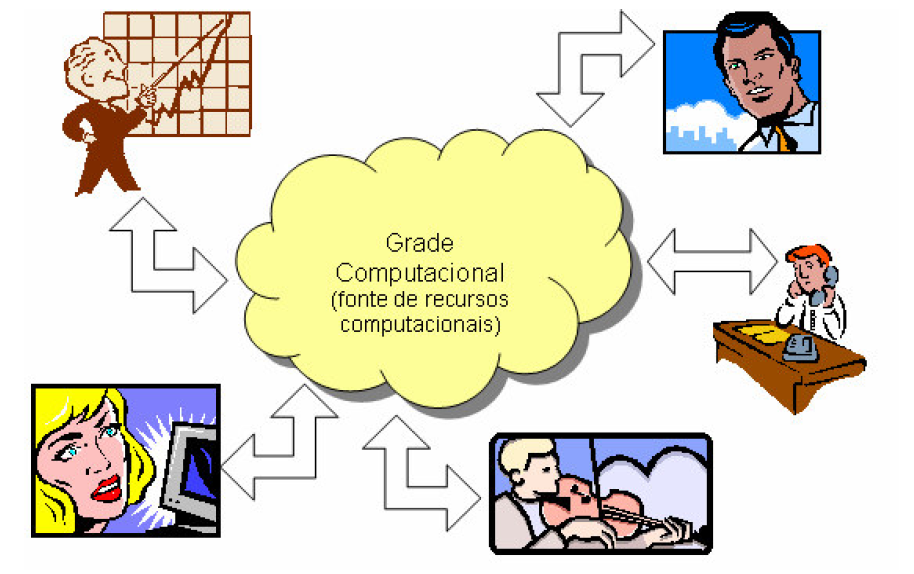
\includegraphics[width=0.6\textwidth]{figuras/grade-comp.png}
% 	% Caption centralizada
% % 	\captionsetup{justification=centering}
% 	% Caption e fonte 
% 	 \vspace{-0.2cm}
% 	\\\textbf{\footnotesize Fonte: \cite{cap-livro} }
% 	\label{fig:figura1}
% \end{figure}
% \vspace{-0.5cm}

% \subsection{\esp Inserção de tela de software}

% Nos casos de telas de \textit{software}, devem ser inseridas como figuras, e referenciadas no texto
% como na Figura \ref{fig:tela1}. Além disso, é necessário que seja citada no texto a empresa desenvolvedora.

% % Figura
% \begin{figure}[!ht]
% 	\centering	
% 	\caption[\hspace{0.1cm}Exemplo de tela de software.]{Exemplo de tela de software}
% 	  \vspace{-0.4cm}
% 	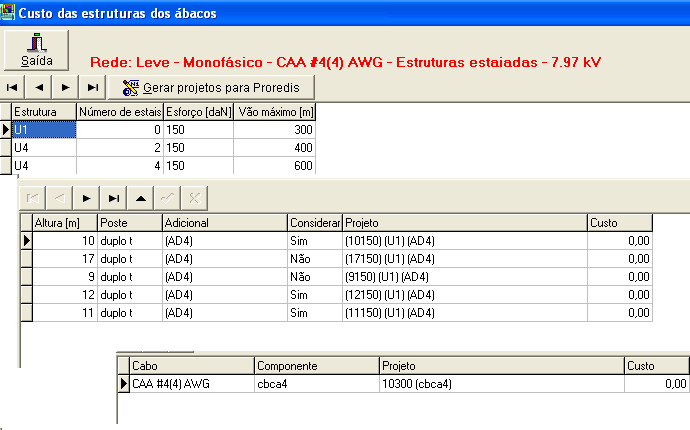
\includegraphics[width=.8\textwidth]{figuras/tela1.png}
% 	% Caption centralizada
% % 	\captionsetup{justification=centering}
% 	% Caption e fonte
% 	 \vspace{-0.3cm}
% 	\\\textbf{\footnotesize Fonte: \cite{tela1}}
% 	\label{fig:tela1}
% \end{figure}

% \subsection{\esp Inserção de gráficos e mapas}

% O gráfico é um tipo de ilustração que deve conter todos os elementos citados e também a descrição de seu título
% diferenciando-o das figuras da mesma forma que no Gráfico 1. 

% \begin{center}
% 	\centering	
%  	\textbf{Gráfico 1 - Exemplo de um gráfico} \\
% %  	  \vspace{0.cm}
% 	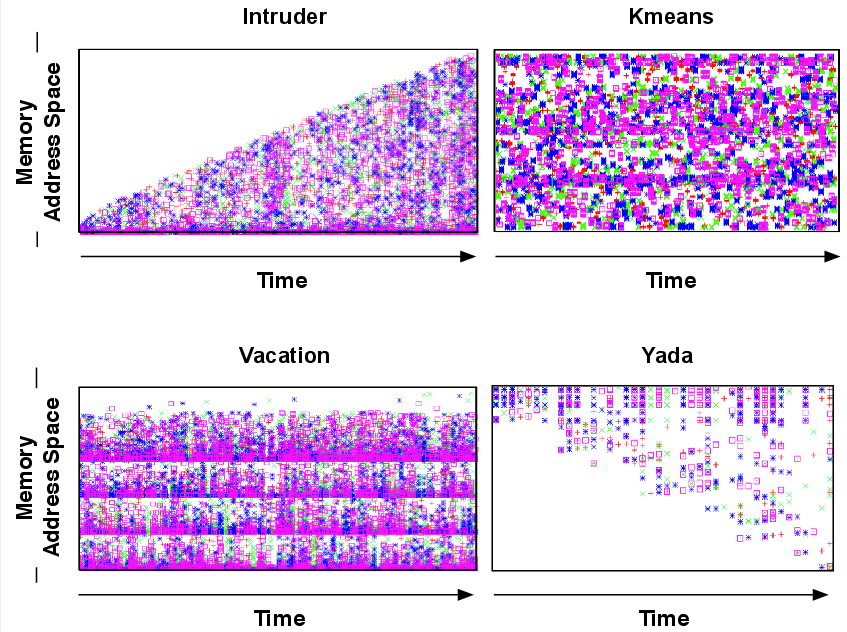
\includegraphics[width=0.7\textwidth]{figuras/access.png}
% 	% Caption centralizada
% % 	\captionsetup{justification=centering}
% 	% Caption e fonte
% 	 \vspace{-0.3cm}
% 	\\\textbf{\footnotesize Fonte: \cite{tese}}
% 	\label{grafico1}
% \end{center}

% A mesma regra se aplica para mapas, que devem ser adicionados seguindo as regras de apresentação já mostradas. No caso específico,
% o título e a numeração, também como os gráficos, devem começar do numeral ``1'' depois da marcação ``Mapa'' seguido do nome do elemento.
% Exemplo: \textbf{Mapa 1 - Exemplo de um Mapa}.

%  \subsection{\esp Tabelas}

% As tabelas devem ser abertas nas laterais, com espaços verticais separando
% as colunas e sem espaços horizontais, exceto na
% separação do cabeçalho. Um exemplo é a Tabela \ref{tab:tabela1}. 

% % Tabela
% \begin{table}[htb]
% 	\centering
% 	\caption{\hspace{0.1cm} Exemplo de uma tabela}
% 	\vspace{-0.3cm} % espaço entre titulo e tabela
% 	\label{tab:tabela1}
% 	% Conteúdo da tabela
% 	\begin{tabular}{l|c|c}
%   \hline
%     \textbf{Imagem}	& \textbf{transferência} & \textbf{tempo} \\
%     \hline
%      estação 1	& 7,72 MB/s &  1:22:18 \\
%      estação 2	& 7,72 MB/s &  1:22:17 \\
%      estação 3	& 7,59 MB/s & 1:24:25 \\
%      estação 4  & 7,53 MB/s & 1:43:27 \\
%      estação 5	& 6,14 MB/s  &  1:24:41 \\
%      estação 6  &  7,50 MB/s & 1:23:53 \\
%      estação 7  & 7,58 MB/s  &  1:24:02 \\
%      estação 8  & 7,8 MB/s  &  1:29:06 \\
%      estação 9  & 7,9 MB/s  &  1:30:05 \\
%      estação 10 & 8,0 MB/s  &  1:32:03 \\
%      \hline
%  \end{tabular}
%  	\vspace{.1cm}  %espaço entre tabela e fonte
% 	\small
% 	% Fonte
% 	{\footnotesize\\ \textbf{Fonte: \cite{monog-fabio}}}
% \end{table}

% \subsection{\esp Quadros}

% Os quadros diferem das tabelas por apresentarem dados textuais.
% Esses dados podem ser esquemáticos, comparativos ou descritivos.

%    \begin{center}
%           \centering
%        	\textbf{Quadro 1 - Bandas/Artistas de Rock e outros}\\
% % 	\vspace{-0.3cm} % espaço entre titulo e tabela
%         \label{quadro1}
% 	\begin{tabular}{|c|c|c|c|} \hline
% 	\multicolumn{4}{|c|}{\textbf{Bandas ou Artigas de Rock e outros}} 	  \\ 
% 		\hline \textbf{	Progressivo} & Pink Floyd & Jethro Tull	& Yesterday \\ 
% 		 \hline \textbf{ Metal}  & Metallica & Iron Maidam & Black Sabath \\ 
% 		\hline \textbf{	Arena Rock} & Led Zeppelin & The Rolling Stones & Beatles \\ 
% 		\hline \textbf{ Punk} & Ramones & Black Flag & NOFX	\\ 
% 		\hline \textbf{	Nacional} & Ira & Engenheiros & Vinil	\\ 
% 		\hline \textbf{	S.J.E.} & Apolo XI & Invasão 7 & Por do Sol \\ 
% 		\hline \textbf{	Grunge} & Nirvana & Pear Jam & Alice in Chains	\\ 
% 		\hline \textbf{	Rock Folk} & Bod Dylan & The Byrds &  The Mamas \& the Papas \\
% 		\hline \textbf{	Blues} & B.B. King & Albert Colins & Mady Wathers \\ 
% 		\hline \textbf{	New Wave} & The Police & The Pretenders, &  Duran Duran\\ 
%  		\hline \textbf{	Rock Folk} & Bod Dylan & The Byrds &  The Mamas \& the Papas \\
%  		\hline \textbf{	Rock alternativo} & R.E.M.& Hüsker Dü & Big Black\\ 
 		
% 		\hline
% 	\end{tabular}
% 	\vspace{0.1cm} 
% 	{\footnotesize\\ \textbf{Fonte: Dados da pesquisa}}
%    \end{center}

% Para gráficos, quadros e tabelas, cujos dados foram extraídos da própria pesquisa, 
%  usar a expressão: Dados da pesquisa. Ver exemplo no Quadro 1.
   

% \subsection{\esp Inserção de algoritmos}

% Para inserir um algoritmo, utilizar o exemplo do Algoritmo  \ref{alg:rnagenerica}.
% Todos os algoritmos devem ser inseridos como figura, indicada por nome e  fonte. Caso 
% forem de própria autoria, isso deverá ser mencionado na fonte, como elaboração feita pelos autores.

% % algoritmo
% % \begin{figure}[ht]
% \begin{center}	
% 	% Arquivo da figura
% % 	\caption[\hspace{0.1cm} Texto da figuras.]{Algorítmo CAC RD Neural}
%          \textbf{Algoritmo 1 -  CAC RD Neural}
% 	\vspace{-0.3cm}
% \begin{minipage}[ht]{13cm}
% \begin{algorithm}[H]
%   \footnotesize
%   \caption{CAC-RD Neural}
%   \label{alg:rnagenerica}
%   \begin{algorithmic}[1]
%       \STATE \textbf{Entrada:} Requisição da chamada
%     \STATE \textbf{Saída:} Aceitação ou bloqueio da solicitação
    
%     \STATE Preenche o vetor de $attributes.size+1$ atributos com os valores dos atributos, sendo a primeira posição do vetor preenchida com o valor 1
% 		\STATE $hidden\_layer\_size =  attributes.size*2+1;$

%     \FOR{$i$ = 1 to $attributes.size+1$}
%     	\STATE \textbf{normalizar}($Entrada_i$)
%     \ENDFOR

% 		\STATE $double [] net = new double [hidden\_layer\_size];$
%     \STATE $net = hidden\_layer\_weights * attributes;$
%    	\FOR{$i$ = 0 to hidden\_layer\_size}
% 			\STATE $net [i] = 1.0 / (1.0 + exp((-1.0)*net[i]));$
% 		\ENDFOR

% 		\STATE $double [] ipVector = new double [hidden\_layer\_size+1];$
%     \STATE $ipVector [0] = 1.0;$
%    	\FOR{$i$ = 1 to $hidden\_layer\_size+1$}
% 			\STATE $ipVector [i] = net [i-1];$
% 		\ENDFOR
		
% 		\STATE $output = output\_layer\_weights *  ipVector;$
%     \STATE output = \textbf{desnormalizar}(Saída)
%     \STATE \textbf{net\_update} (requisition);
    
%     \STATE \textbf{Retorna} output; FIM
%   \end{algorithmic}
% \end{algorithm}
% % \vspace{-0.3cm} % espaço entre algoritmo e fonte

% \small \centering \textbf{\footnotesize Fonte: \cite{mestrado}.}
% \end{minipage}
% \end{center}
% % \end{figure}

% Para ilustrações criadas ou adaptadas a partir de outras ilustrações, usar as expressões: 
% “Adaptado de...” ou “Criado pelo autor`` com dados extraídos de \ldots
   
   
% \section{\esp CITAÇÕES}


% Referências deverão ser adicionadas no arquivo \textit{bibliografia.bib}. Cada referência deverá ser adicionada conforme o padrão de normalização da PUC, 
% o qual poderá ser consultado na página da biblioteca da PUC Minas \cite{manualpuc}. Todas as publicações citadas no texto deverão ter correspondente nas referências, 
% e as indicações de autoria da citação e do ano deverão ser idênticas aos dados expostos.


% \subsection{\esp Citação livre ou indireta}

% Quando se reproduzir ideias, sem transcrever as palavras do autor, a indicação da página é opcional. Exemplos desse tipo de citação:
% \begin{enumerate} 
%  \item [a)] Citação com um autor \cite{knuth}. 
%  \item [b)] Citação de artigos em revistas com dois autores \cite{artigo01}.
%   \item [c)] Trabalho em congresso com três autores \cite{dovzan:01}.
%  \item [d)] Trabalhos com mais de três autores \cite{cap-livro}.
%  \item [e)] Dois autores em duas obras distintas \cite{knuth,groupp}.
%  \item [d)] Trabalhos distintos com vários autores \cite{congresso,cap-livro}.
 
% \end{enumerate}

% \subsection{\esp Citação direta ou textual}

% Transcrição literal de textos de outros autores. Nesse caso, deverão ser especificadas as páginas consultadas. 
% Se desejar, poderão ser grafadas em itálico para melhor visualização.

% \subsubsection{\esp Textual Curtas}

% Quando curtas (até 3 linhas) serão inseridas na sequência normal do texto, entre aspas com as mesma formatação.

% \subsubsection{\esp Textual Longas}

% Citações longas (mais de 3 linhas) deverão constituir um parágrafo independente, recuado a 4 cm da margem esquerda, 
% com letra tamanho 10 e digitado em espaço simples, sem aspas.
% \begin{citacaodireta}
% Hegel chama trabalho à forma específica da satisfação das necessidades, que
% distingue da natureza o espírito existente. Assim como a linguagem infringe
% a imposição da intuição e ordena o caos das múltiplas sensações em coisas
% identificáveis, assim o trabalho infringe a imposição do \hspace{0.1cm}desejo \hspace{0.1cm}imediato \hspace{0.1cm}e
% suspende, por assim dizer, o processo de satisfação das necessidades.
% \cite[25]{habermas}.
% \end{citacaodireta}


% % Artigo \cite{whatershed:01}

% \subsubsection{\esp Textual de outros idiomas (Tradução)}

% \begin{citacaodireta} 
% Um \textit{cluster} é um computador paralelo construído de componentes e processos de \textit{software} (tal como sistema de \textit{software}). 
% Um \textit{cluster} é formado de nós, cada um contendo um ou mais processadores, memória que é compartilhada por todos os processadores do nodo 
% (somente eles), e dispositivos periféricos adicionais (tais como discos), conectados pela rede e que permitem tráfego de dados entre os nós...
% \cite[p. 10, tradução nossa]{groupp}\footnote {  … a cluster is a parallel computer that is constructed of commodity  componets and runs 
% (as its system software) commodity software. A cluster is made of nodes, each conteining one or more processors, memory that is  shared 
% by all of the processors in (and only on) the node, and addtional peripheral devices (surch as disks),
%  connected by network that allows data to move between the nodes}.
% \end{citacaodireta}
 
% \subsection{\esp Exemplos de citações} 

% Alguns exemplos de citações mais utilizadas e/ou que geram algumas dúvidas. É válido observar que não citaremos
% todas as possibilidades de citações da norma da PUC Minas, sendo assim é de extrema relevância que se consulte 
% o documento no site da Biblioteca da PUC Minas para maiores esclarecimentos acerca de citações \cite{manualpuc}.

% \subsubsection{\esp Citação de monografia, dissertação e tese}

% Exemplo de citação de monografia de curso de graduação ou especialização pode ser vista em \citeonline{monog-fabio}.
% Exemplo de dissertação de mestrado é referida como \citeonline{mestrado}.

% Para o caso de doutorado é citado da seguinte forma, Góes (\citeyear{tese}). Nesse exemplo é válido observar a forma
% como está escrito no documento \LaTeX, pois citações que compreendem no texto o nome do autor como sua parte, necessitam 
% do parâmetro \verb$\citeonline{}$. 

% \subsubsection{\esp Livros e partes de livros}

% Exemplo de capítulo de livro fica conforme este exemplo \cite{cap-livro}.

% Para livros citados no corpo do texto e com duas citações juntas, ver os exemplos \citeonline{knuth,groupp}.
% Caso essa citação não fizesse parte do texto será referencia dessa forma \cite{knuth,groupp}.

% Citações institucionais ou documentos técnicos de alguma entidade devem ser citados desta forma \cite{pmbok}.

% \subsubsection{\esp Tela de software}

% Para  citar a tela de um \textit{software} faça da seguinte forma, \citeonline{tela1}.

% \subsubsection{\esp Citações da Biblia Sagrada}

% A Bíblia está dividida em duas grandes partes: O Antigo Testamento e o Novo Testamento, divididos em livros, capítulos e versículos. 
% Portanto, a citação de partes da Bíblia deve apresentar o título do livro de forma abreviada ou por extenso, o número do capítulo e o número do versículo.


% \begin{citacaodireta}
% Moisés estendeu a mão sobre o mar. Com um forte \hspace{-0.1cm} vento \hspace{0.1cm} leste a \hspace{0.1cm}sobrar a
% noite toda, o Senhor repeliu o mar e o pôs a seco. As águas se fenderam e
% os filhos de Israel entraram no meio do mar a pé enxuto, enquanto as águas
% formavam uma muralha à direita e à esquerda deles (\citeauthor{biblia} 14,21).
% \end{citacaodireta}

% \subsection{\esp Conclusão}

% Discussão dos resultados obtidos na pesquisa. É onde se colocam as observações do autor. 
% Poderá também apresentar sugestões de novas linhas de estudo.

% A conclusão deve estar de acordo com os objetivos do trabalho.

% A conclusão não deve apresentar citações ou interpretações de outros autores.

%\section{\esp Introdução \label{introducao}}

%considerações iniciais
O \ac{SAD} caracteriza-se como uma modalidade de assistência à saúde prestada em domicílio composta por um conjunto de ações de prevenção, reabilitação e tratamento de doenças.
Esse tipo de serviço tem se tornado cada vez mais presente, oferecendo uma forma alternativa de atendimento às pessoas com quadro clínico estável e que necessitam de cuidados especializados, substituindo a internação hospitalar.

Essa modalidade de assistência a saúde oferece maior comodidade aos pacientes, garantindo maior conforto, facilitando o apoio familiar, além de reduzir riscos de contaminação hospitalar e a lotação dos leitos nos hospitais.
Por outro lado, o~\ac{SAD} apresenta alguns desafios para os profissionais de saúde, tais como a necessidade de deslocamento dos profissionais de saúde de forma  que todos os pacientes que estejam agendados para determinado dia sejam atendidos no tempo previsto, além do complexo planejamento das escalas de trabalho dos profissionais de saúde envolvidos no atendimento domiciliar \citeonline{Kergosien:2009}. 
Visando atender pacientes em domicílio, é necessário definir rotas a serem seguidas pelos veículos do~\ac{SAD}, pois os caminhos a serem percorridos podem depender de alguns fatores, tal como a necessidade de urgência de algum paciente. 

Devido ao complexo planejamento das escalas de trabalho dos profissionais e as dificuldades encontradas para completar todo o serviço diário no tempo previsto, sem exceder a carga horária dos profissionais de saúde. Dessa forma, o \ac{SAD} tem despertado o interesse de diversos pesquisadores, que definiram o problema relacionado à modalidade estudada como \ac{PERE}.
O \ac{PERE} aborda de forma integrada o problema de roteamento de veículos e de escalonamento de enfermeiras, com o objetivo de desenvolver um cronograma de trabalho para o \ac{SAD}, de forma que cada enfermeira visite um conjunto de pacientes, faça uma pausa e finalize suas atividades previstas dentro de uma janela de tempo de trabalho pré definida. \cite{trabelsi:2012}. 
Para satisfazer as restrições do \ac{PERE}, além de definir a escala de trabalho dos profissionais, é necessário definir rotas que serão seguidas pelos veículos do~\ac{SAD}, uma vez que a elaboração dos trajetos que serão seguidos dependem de alguns fatores, tal como a necessidade de urgência de algum paciente. 

%Segundo \cite{Kergosien:2009} é possível reduzir o PERE ao Problema dos Múltiplos Caixeiros Viajantes, dessa forma, pode-se classificar o \ac{PERE} na classe de problemas NP-Difícil, portanto, é pouco provável que seja possível determinar um algoritmo polinomial para resolve-lo.
Segundo \citeonline{Kergosien:2009} é possível reduzir o PERE ao Problema dos Múltiplos Caixeiros Viajantes, classificando-o então na classe de problemas NP-Difícil. Portanto, é pouco provável que seja possível determinar um algoritmo polinomial para resolve-lo.
Apesar disso, de acordo com \citeonline{cheng:98}, \citeonline{bachouch:2010},\citeonline{tozlu:2016} e \citeonline{cattafi:2012}, o \ac{PERE} ainda é resolvido de forma manual em diversos países, o que pode acarretar em resultados insatisfatórios. 
Por fim, é estimado em \citeonline{holm:2014} que os profissionais envolvidos no \ac{SAD} passam entre $18\%$ e $26\%$ da sua jornada de trabalho dentro do veículo realizando translados entre os pontos de atendimento, o que reforça a necessidade da utilização de técnicas de otimização como forma de abordagem.

Devido a natureza do problema, diversos métodos para encontrar a melhor solução para o \ac{PERE} são encontrados na literatura. Com o objetivo de investigar de maneira formalizada, quais métodos vêm sendo desenvolvidos para solucioná-lo, encontrar  possíveis problemas de investigação existentes, garantindo a replicabilidade desta revisão e  auxiliando outros pesquisadores do tema no momento da obtenção de materiais de estudo, elaboramos uma \ac{RSL}.

%Para verificar a necessidade da elaboração de uma \ac{RSL}, foram elaboradas pesquisas para buscar a existência de outra revisão da mesma natureza. 
Nas pesquisas realizadas não foram encontradas outras \ac{RSL}, mas foram encontradas outras revisões de literatura, classificadas por \citeonline{Kitchenham:2007} como ad-hoc,  publicadas por \citeonline{fikar:2017} e \citeonline{mohamed:2017}.

\subsection{\esp Revisões de Literatura Recentes}
%revisões de literatura existentes

A revisão de literatura escrita por \citeonline{fikar:2017} tem como propósito comparar diferentes objetivos, restrições e destacar as pesquisas futuras para o \ac{PERE}, para isto os autores compararam diversos artigos, até Outubro de 2015, não indicando a data do início da sua pesquisa. As buscas foram realizadas pelos autores a partir seguintes palavras chave: \textit{``Home Care'', ``Home Health Care'', ``Routing'' e ``Rcheduling''}. 
A revisão de literatura desenvolvida por \citeonline{mohamed:2017} tem como objetivo analisar a literatura existente relativa ao \ac{PERE}, para isso o autor comparou  materiais de diferentes naturezas, tais como artigos científicos, capítulos de livros, teses, dissertações e relatórios técnicos, publicados entre 1997 e 2015, a partir das seguintes palavras chave: \textit{ ``Home Health Care'', ``Home Care'' ``Resource  Scheduling'',  ``Routing'' e ``Vehicle Routing Problem"}

A partir dos resultados obtidos em sua revisão, foi afirmado por \citeonline{fikar:2017} que o \ac{PERE} foi primeiro estudado em 1974 a partir do artigo \textit{A Model for Community Nursing in a Rural County}, publicado por \citeonline{fernandez:1974}. Em suas pesquisas \citeonline{fikar:2017}, verificaram  que alguns artigos estão diretamente relacionados com o \ac{PRV} e as restrições mais consideradas incluem janelas de tempo, requisitos de habilidades e de tempo de trabalho.
\citeonline{fikar:2017} destacaram, as seguintes técnicas de solução aplicadas ao \ac{PERE}: \textit{Adaptative Large Neighborhood Search, Variable Neighborhood Search, Branch and Price and cut, Discrete-Event-Simulation, Greedy Randomized Adaptive Search Procedure, Fuzzy Simulated Evolution Algorithm, Genetic Algorithm, Memetic Algorithm, Multi-Directional Local Search, Particle Swarm Optimization, Repeated Matching, Simulated Annealing, Scatter Search e Tabu Search}.

\citeonline{mohamed:2017} classificaram as restrições relacionadas aos pacientes, a organização e aos profissionais como: temporais, de associação e geográficas. 
Para os pacientes, as restrições temporais determinam a frequência de visitas, a janela de tempo do atendimento e as dependências temporais; as restrições de associação determinam as preferências dos pacientes, tais como: ser atendido sempre pela mesma enfermeira; as restrições geográficas estão associadas a localização do paciente, e são utilizadas para auxiliar no cálculo de estimativa de tempo de viagem. 
Para a organização, as restrições temporais são utilizadas para realizar o planejamento de tempo; as restrições de associação são utilizadas para garantir a continuidade dos atendimentos até o final do tratamento; e as restrições geográficas são utilizadas para determinar a área de atendimento. 
Para os profissionais, as restrições temporais são utilizadas para determinar as horas trabalhadas; as restrições de associação são determinadas a partir das habilidades de cada enfermeira; e as restrições temporais são utilizadas para determinar o local de cada atendimento.

%por que elas não são revisões sistemáticas
Apesar do trabalho publicado por \citeonline{fikar:2017} e \citeonline{mohamed:2017} descreverem as palavras chave utilizadas na elaboração da pesquisa, o limite superior de tempo no qual as pesquisas foram consideradas, as palavras chave utilizadas na pesquisa e da revisão publicada por \citeonline{mohamed:2017} definir os motores de busca que foram utilizados. 
Segundo \citeonline{Kitchenham:2007}, ambos os trabalhos são classificados como revisões de literatura ad-hoc, pois não foram elaborados seguindo um protocolo formal para realizar a busca dos materiais, possuem objetivos abrangentes, não existe uma questão de pesquisa a ser respondida ao final da revisão, não foram elaboradas strings de busca nem critérios para inclusão e exclusão dos estudos retornados na pesquisa. 

Além da Revisão Sistemática de Literatura, este artigo traz como contribuição materiais não retornados na busca das revisões pesquisadas anteriormente, além de enfatizar estudos de caso relevantes desenvolvidos por pesquisadores em conjunto com o governo local ou empresas privadas e destacar as métricas e metodologias mais empregadas por pesquisadores para solucionar o \ac{PERE}.

%organização do artigo

Este artigo está organizado da seguinte forma:  Na Seção~\ref{protocolo} é apresentado o protocolo da revisão sistemática de literatura. Na Seção~\ref{terminologia}  são apresentadas as terminologias relacionadas ao PERE que são utilizadas também ao longo do texto. Na Seção~\ref{pad} são apresentadas as métricas utilizadas para avaliar as soluções do \ac{PERE}. Na Seção~\ref{metodologia}  foram descritas as metodologias mais utilizadas. Na Seção~\ref{aplicacoes} são apresentados os comparativos do \ac{PERE} com outros problemas. Na Seção~\ref{casos} listamos alguns estudos de casos e discutimos alguns problemas com características únicas, e finalizando o artigo, na Seção~\ref{conclusão} são apresentadas as considerações finais.








%\section{\esp Protocolo da Revisão Sistemática de Literatura }\label{protocolo}

%Definição, diferença
Segundo \citeonline{Kitchenham:2007}, uma \ac{RSL} é um método de seleção de artigos, no qual a busca por materiais bibliográficos é formalizada sistematicamente a partir da elaboração e utilização de um protocolo de busca. Uma \ac{RSL} tem como objetivos: resumir evidências empíricas, identificar lacunas existentes nas pesquisas realizadas até o momento e fornecer subsídios para realizar novas pesquisas.
Enquanto uma Revisão Literatura, também chamada de Revisão Ad-hoc, não utiliza o protocolo para a formalização da pesquisa realizada, dessa forma tornando mais difícil sua replicabilidade.

%etapas
Uma \ac{RSL} é  composta por três fases: planejamento da revisão, condução da revisão e análise dos materiais obtidos.
Na fase de planejamento define-se a pergunta de pesquisa, seleciona-se as palavras chave e determina-se os critérios de inclusão e de exclusão de materiais bibliográficos; na condução da revisão é realizado uma busca a partir da combinação das palavras chave e na última fase  é realizado um estudo dos materiais que foram obtidos. A seguir será apresentada a descrição das etapas da elaboração e a execução do protocolo de \ac{RSL} utilizado neste artigo para encontrar e selecionar os materiais que posteriormente foram estudados neste artigo.

%Protocolo da revisão
\subsection{Planejamento da Revisão}

A revisão sistemática de literatura proposta neste trabalho tem como objetivo investigar quais métricas e metodologias aplicadas ao \ac{PERE} entre 1998 e o mês de Outubro de 2016, abrangendo um período de 18 anos, de forma a responder a seguinte questão de pesquisa:

\begin{itemize}
\item \emph{Quais métricas e metodologias empregadas ao \acl{PERE} foram publicadas desde 1998 até o mês de Outubro de 2016?}
\end{itemize}

Para responder à pergunta foram consultados artigos de pesquisadores que aplicaram métricas e metodologias ao \ac{PERE}, tendo como um dos resultados esperados a relação das métricas e metodologias utilizadas no período de tempo definido na questão anterior. 

A consulta por artigos relacionados foi realizada com a utilização das seguintes palavras chave:

\begin{itemize}
\item \textit{``home health care''}
\item \textit{``home care''}
\item \textit{``nurse''}
\item \textit{``routing''}
\item \textit{``scheduling''}
\end{itemize}

Organizadas na seguinte expressão de busca:

\begin{itemize}
\item \textit{`` ( (``home health care'' OR ``home care'' OR ``nurse'') AND ``routing'' AND ``scheduling'' ) ''}
\end{itemize}

Após a elaboração da expressão de busca, foram definidos os critérios para inclusão e exclusão dos materiais bibliográficos.

\textbf{Critérios de inclusão:}

\begin{itemize}
\item Artigos relacionados ao Problema de Escalonamento e Roteamento de Enfermeiras; 
\item Artigos publicados em revistas ou conferências;
\item Artigos completos.
\end{itemize}

\textbf{Critérios de exclusão:}

\begin{itemize}
\item Artigos que foram publicados em idiomas que diferem do inglês ou português;
\item Artigos inacessíveis ou indisponíveis;
\item Artigos duplicados;
\item Artigos publicados antes de 1998.
\end{itemize}

\subsection{\esp Condução das buscas}

Após a definição dos critérios de inclusão e de exclusão dos materiais bibliográficos, foram escolhidas as seguintes bases de pesquisa, a partir da sua popularidade, para realizar as buscas:

\begin{itemize}
\item \textit{Science Direct};
\item \textit{Springer};
\item \textit{Scopus};
\item \textit{IEEE Xplore};
\item \textit{ACM Digital Library}.
\end{itemize}

Após a realização das buscas, foram retornados 158 resultados, organizados na Figura~\ref{bases}. 

\begin{figure}[ht]
\begin{center}
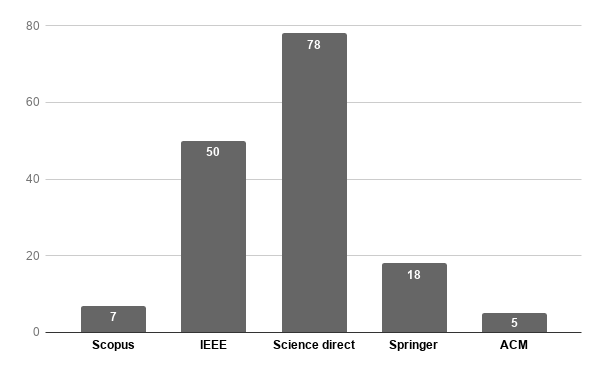
\includegraphics[width=0.4\textwidth]{base_de_dados_de_origem.png}
\caption{Contagem por bases de pesquisa \label{bases}}
\end{center}
\end{figure}


A partir da aplicação dos critérios de inclusão e de exclusão nos artigos consultados foram aceitos 19 artigos, por atenderem a todos os critérios de inclusão e 139 artigos rejeitados por atenderem a pelo menos um critério de exclusão ou por não se encaixarem em algum critério de inclusão. É interessante observar que os artigos coletados foram publicados entre os anos de 1998 e 2016, sendo que houve um aumento considerável de publicações entre os anos de 2012 e 2016, de acordo com a Figura~\ref{ano}.
 
Após a aplicação dos critérios de inclusão e exclusão nos materiais bibliográficos, foi observado que 86,7\%,  dos artigos foram rejeitados. Acredita-se que o motivo para este alto índice de rejeição seja por conta da relação do assunto estudado com publicações existentes em diversas áreas de saúde, fazendo com que as bases de pesquisa apontassem para artigos que posteriormente não se encaixariam em algum critério de inclusão. 

\begin{figure}[ht]
\begin{center}
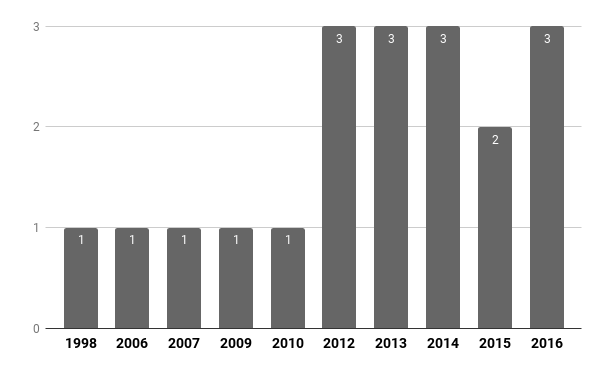
\includegraphics[width=0.4\textwidth]{contagem_por_ano.png}
\caption{Contagem de artigos por ano de publicação \label{ano}}
\end{center}
\end{figure}



% \subsection{\esp Trabalhos futuros}
% 
% Sugestões de estudos posteriores são ser adicionados subseção deste capítulo de conclusão.